The purpose of our algorithm is to make a three dimensions tracking system, producing position informations 
about a followed target (ROI).
The information will be relevant to define parameters 
as: the relative velocity, the factor of approaching and of departure.

The proposed algorithm is shown in Fig. \ref{fig:system};
it begins with a key frame image where a initial target is determined; 
the system then receives a stream of image frames and the tracking system 
enters into looping follow this target in the next frames.

\begin{figure}[bhp]
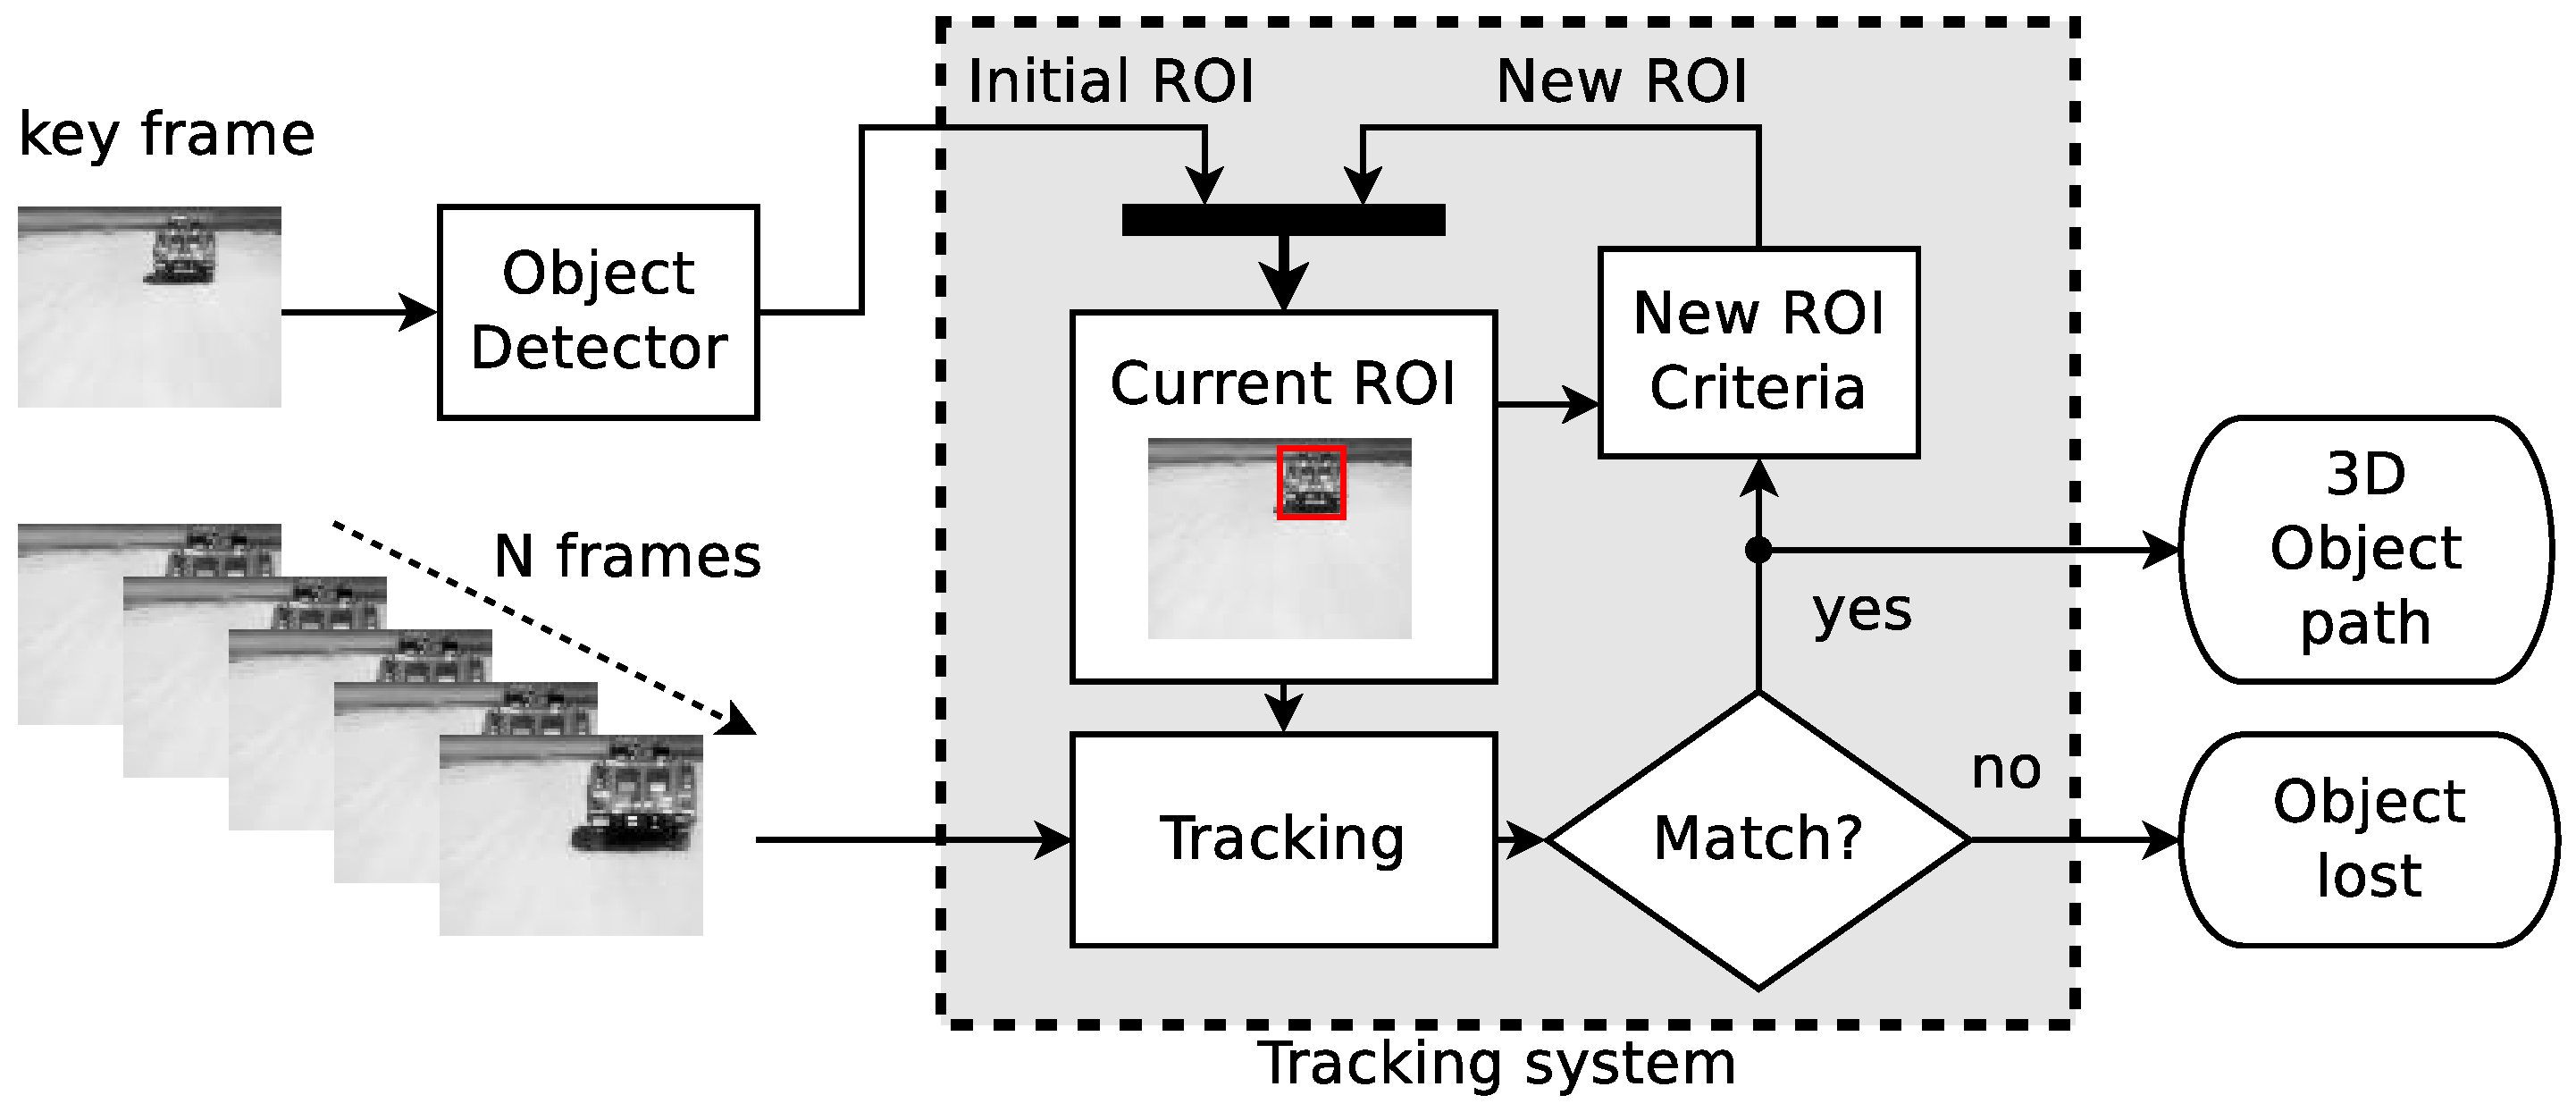
\includegraphics[width=\columnwidth]{images/figure1-diagram1.eps}
\caption{The target is identified from a highest value of correlation (PCC) between a selected ROI and 
the Window Of Search (WOS) of a current frame; the result of this process is a displacement which is  returned as vector field.}
\label{fig:system}
\end{figure}

In a two dimensional analysis, the tracked target given us information about its horizontal 
and vertical position and its relative perpendicular velocity with respect to the observer.
When the target is analysed in three dimensions, 
the initial $ROI$ has the position $(x=x_0,y=x_0,d=d_0=1)$;
where, $x_0$ and $y_0$ represent a position (horizontal and vertical) in the analysed image,
and $d_0=1$ represents the initial depth position of target in the $ROI$ (normalized by definition to $1.0$).
Thus, all the results of depth will be relative to this value. In this sense, the relative velocity and 
the factor of approaching or departure can be calculated.

%Diagrama1
 %A gente vai explicar o algoritmo como uma caixa fechada , que coisa entra e que coisa sai
 %e os parametros a sintonizar.
 % como usar ele quando implementado, como se fosse uma caixa preta.
